\documentclass[12pt]{article}
\usepackage[english]{babel}
\usepackage{natbib}
\usepackage{url}
\usepackage{hyperref}
\usepackage{minted}
\usemintedstyle{borland}
\usepackage{listings}
\usepackage[utf8x]{inputenc}
\usepackage{graphicx}
\graphicspath{{images/}}
\usepackage{fancyhdr}
\usepackage{vmargin}
\setmarginsrb{3 cm}{2.5 cm}{3 cm}{2.5 cm}{1 cm}{1.5 cm}{1 cm}{1.5 cm}
%%%%%%%%%%%%%%%%%%%%%%%%%%%%%%%%%%%%%%%%%%%%%%%%%%%%%%%%%%%%%%%%%%%%%%%%%%%%%%%%%%%%%%%%%
\title{Práctica 5: Pipes \& Fork}% Title 
\author{Meza Madrid Damián}% Author
\date{Abril 2019}% Date
%%%%%%%%%%%%%%%%%%%%%%%%%%%%%%%%%%%%%%%%%%%%%%%%%%%%%%%%%%%%%%%%%%%%%%%%%%%%%%%%%%%%%%%%%
\makeatletter
\let\thetitle\@title
\let\theauthor\@author
\let\thedate\@date
\def\@seccntformat#1{%
\expandafter\ifx\csname c@#1\endcsname\c@section\else
\csname the#1\endcsname\quad
\fi}
\makeatother
\pagestyle{fancy}
\fancyhf{}
\rhead{\theauthor}
\lhead{\thetitle}
\cfoot{\thepage}
\begin{document}

%%%%%%%%%%%%%%%%%%%%%%%%%%%%%%%%%%%%%%%%%%%%%%%%%%%%%%%%%%%%%%%%%%%%%%%%%%%%%%%%%%%%%%%%%

\begin{titlepage}
	\centering
    \vspace*{0.5 cm}
    
\includegraphics[scale = 0.30]{escom.png}\\[1.0 cm]	% University Logo
	\textsc{\Large Instituto Politécnico Nacional}\\[0.5 cm]% Course Code
	\textsc{\Large Escuela Superior de Computo}\\[0.5 cm]% Course Code
	\rule{\linewidth}{0.2 mm} \\[0.4 cm]
	{ \huge \bfseries \thetitle}\\
	\rule{\linewidth}{0.2 mm} \\[1.5 cm]
	Reporte\\
	Profesor: Ulises Velez Saldaña \\
	Alumno: Meza Madrid Raúl Damián\\
    Clase: Sistemas operativos\\
    Grupo: 2CM7\\
\end{titlepage}
\tableofcontents
\pagebreak
\section{Introducción}
\subsection{Procesos}
La principal entidad activa en un sistema Linux es el proceso . Linux es un sistema multiprograma , por lo tanto, múltiples procesos independientes pueden estar corriendo al mismo tiempo. Los procesos son creados en  una manera simple. El proceso que ejecuta la llamada al sistema \emph{fork} se llama proceso padre. El nuevo proceso es llamado proceso hijo. El padre y el hijo tienen su propia memoria privada. Si el padre si el padre subsecuentemente cambia cualquiera de sus variables, los cambios no son reflejados en el hijo y vice versa. 
\subsection{Pipe}
Un pipe es una especia de pseudo archivo que puede ser usado para conectar dos procesos. Si un proceso A y N desean comunicarse usando un pipe, necesita escribir y leer del pipe como si fuera un archivo de entrada y salida, de esta manera la comunicación entre dos procesos dentro de UNIX se ve muy similar a una lectura/escritura en archivos. 
\subsection{Programas y herramientas utilizados}
Esta práctica fue desarrollada en el sistema operativo Ubuntu 18.04.1 LTS. Estos son los programas y herramientas utilizados, junto con el comando de instalación, en caso de que no estuvieran instalados ya. 
\begin{itemize}
    \item Doxygen 
    \begin{minted}{bash}
        git clone https://github.com/doxygen/doxygen.git
        cd doxygen
        mkdir build
        cd build
        cmake -G "Unix Makefiles" ..
        make
        make install
    \end{minted}
    \item make
    \item cmake
    \item python
\end{itemize}
\section{Objetivo}
Que el alumno aplique la teoría vista en clase implementando la comunicación entre un proceso y sus hijos a través de distintos pipelines. Para esto se creara un programa en C que generará \emph{n} números aleatorios, escribirá los pares en el pipe para un proceso hijo que se encargara de sumarlos y después lo regresa al proceso padre para que el lo imprima, hará lo mismo para un proceso encargado de los números impares.
\section{Desarrollo}
El primer paso es leer los números del parámetro argv[ ]. Se generaran los n números, después se decidira cuales se escriben en que pipe.\\ Será necesario mantener seguimiento del numero de pares e impares que existen para que cada hijo sepa cuantas veces leer.\\Para lograr la comunicación con ambos procesos se generaran dos pipes correspondientes; pipeImp para los números impares y pipePar para los números pares, tal y como se muestra en el siguiente diagrama.
\begin{figure}[!htb]
    \centering
    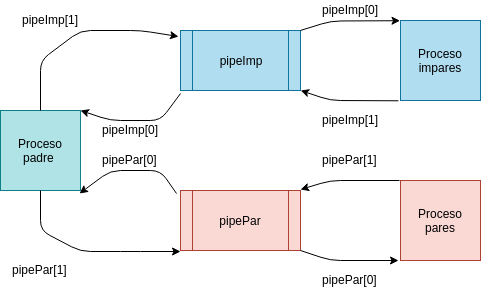
\includegraphics[width=\textwidth*2/3]{pipes.png}
    \caption{Comunicación entre proceso padre(izquierda) e hijos (derecha)}
    \label{fig:listas}
\end{figure}
\pagebreak
\subsection{Codigo}
El codigo fuente contiene comentarios que describen el programa. Son utilizados tambien para documentar con doxygen.
\subsubsection{Código fuente}
\begin{minted}[breaklines,mathescape, linenos, numbersep=5pt, frame=single, numbersep=5pt, xleftmargin=0pt]{c}
#include <stdio.h>
#include <stdlib.h>
#include <unistd.h>
#include <sys/wait.h>
#include <time.h>

int main(int argc, char const *argv[]) {
  /// Se crean los dos pipes y las variables auxiliares par leer y guardar la suma de los numeros pares e impares. Si alguno falla, termina el programa
  /// \code
  int buf ;
  int pipePar[2], sumpar=0, parC=0;
  int pipeImp[2], sumimp=0, impC=0;
  if (pipe(pipePar)==-1 || pipe(pipeImp)==-1) {
    printf("Error al crear los pipes \n");
    return 1;
  }
  /// \endcode

  /// Se crea un arreglo de integers de tamano igual al primer parametro en argv[]
  /// \code
  char *p;
  int n  = strtol(argv[1],&p,10);
  int *nums = (int*)malloc(sizeof(int)*n);
  srand(time(NULL));
  for (unsigned char i = 0; i < n; i++) {
    nums[i]=rand()%10;
    if (nums[i]%2) {
      impC++;
    }else{
      parC++;
    }
    printf("Padre (%d): num alteatorio %d: %d\n",getpid(),i+1,nums[i]);
  }
  /// \endcode

  /// El padre hace 2 forks
  /// \code
  pid_t cpid;
  cpid = fork();
  if (cpid<0) {
    return 1;
  }
  if (cpid) {
    cpid = fork();
      if (cpid<0) {
        return 1;
      }
  /// \endcode

  /// Despues el padre escribe los numeros en su pipe correspondiente
  /// \code
      if (cpid) {
        for (size_t i = 0; i < n; i++) {
          if (nums[i]%2==0) {
            write(pipePar[1],&nums[i], sizeof(int));
          }else{
            write(pipeImp[1],&nums[i], sizeof(int));
          }
        }
  /// \endcode

  /// Cierra los pipes y espera una respeusta
  /// \code
        close(pipePar[1]);
        close(pipeImp[1]);
        wait(NULL);
        wait(NULL);
  /// \endcode

  /// Se leen e imprimen la respuestas correspondientes de cada pipe , despues se cierran
  /// \code
        read(pipePar[0],&sumpar, sizeof(int));
        close(pipePar[0]);
        printf("Padre (%d): Suma pares %d \n",getpid() ,sumpar);
        read(pipeImp[0],&sumimp, sizeof(int));
        close(pipeImp[0]);
        printf("Padre (%d): Suma impares: %d \n",getpid(), sumimp);
        /// \endcode

        /// El segundo hijo (innermost) se dedica a sumar los numeros pares segun el contador, cierra el pipe despues.
        /// \code
      }else{
        for (size_t i = 0; i < parC; i++) {
          read(pipePar[0],&buf, sizeof(int));
          printf("Hijo de pares(%d) : sumando %d \n",getpid(),buf );
          sumpar += buf;
        }
        close(pipePar[0]);
  /// \endcode

  /// Escribe el resultado en el pipe, cierra el pipe y termina el proceso hijo con estado (EXIT_SUCCESS); para que el padre salga de wait(NULL)
  /// \code
        write(pipePar[1], &sumpar, sizeof(sumpar));
        close(pipePar[1]);
        exit(EXIT_SUCCESS);
      }
  /// \endcode

  /// El el primer hijo hace lo mismo, pero para sus numeros correspondientes (impares)
  /// \code
    }else{
      for (size_t i = 0; i < impC; i++) {
        read(pipeImp[0],&buf, sizeof(int));
        printf("Hijo de impares(%d) : sumando %d \n",getpid(),buf );
        sumimp += buf;
      }
      close(pipeImp[0]);
      write(pipeImp[1], &sumimp, sizeof(sumimp));
      close(pipeImp[1]);
      exit(EXIT_SUCCESS);
  }
  /// \endcode
  return 0;
}

\end{minted}
\section{Resultados}
El programa funciona de manera adecuada. A continuacion se muestran dos test case para ilustrar la salida del programa.
\subsection{Caso de prueba: 5}
\begin{minted}[breaklines,mathescape, numbersep=5pt,linenos, frame=single, numbersep=5pt, xleftmargin=0pt,]{bash}
Padre (10583): num alteatorio 1: 5
Padre (10583): num alteatorio 2: 2
Padre (10583): num alteatorio 3: 5
Padre (10583): num alteatorio 4: 7
Padre (10583): num alteatorio 5: 2
Hijo de impares(10584) : sumando 5 
Hijo de impares(10584) : sumando 5 
Hijo de impares(10584) : sumando 7 
Hijo de pares(10585) : sumando 2 
Hijo de pares(10585) : sumando 2 
Padre (10583): Suma pares 4 
Padre (10583): Suma impares: 17 
\end{minted}

\subsection{Caso de prueba: 15}
\begin{minted}[breaklines,mathescape, numbersep=5pt,linenos, frame=single, numbersep=5pt, xleftmargin=0pt,]{bash}
Padre (10641): num alteatorio 1: 6
Padre (10641): num alteatorio 2: 5
Padre (10641): num alteatorio 3: 0
Padre (10641): num alteatorio 4: 9
Padre (10641): num alteatorio 5: 9
Padre (10641): num alteatorio 6: 2
Padre (10641): num alteatorio 7: 0
Padre (10641): num alteatorio 8: 9
Padre (10641): num alteatorio 9: 7
Padre (10641): num alteatorio 10: 3
Padre (10641): num alteatorio 11: 3
Padre (10641): num alteatorio 12: 7
Padre (10641): num alteatorio 13: 8
Padre (10641): num alteatorio 14: 9
Padre (10641): num alteatorio 15: 3
Hijo de impares(10642) : sumando 5 
Hijo de impares(10642) : sumando 9 
Hijo de impares(10642) : sumando 9 
Hijo de impares(10642) : sumando 9 
Hijo de impares(10642) : sumando 7 
Hijo de impares(10642) : sumando 3 
Hijo de pares(10643) : sumando 6 
Hijo de impares(10642) : sumando 3 
Hijo de impares(10642) : sumando 7 
Hijo de pares(10643) : sumando 0 
Hijo de impares(10642) : sumando 9 
Hijo de pares(10643) : sumando 2 
Hijo de impares(10642) : sumando 3 
Hijo de pares(10643) : sumando 0 
Hijo de pares(10643) : sumando 8 
Padre (10641): Suma pares 16 
Padre (10641): Suma impares: 64 
\end{minted}
Cabe notar que en el ultimo ejemplo se puede apreciar como los procesos hijos están corriendo de manera simultanea.
\section{Errores y problemas}
La primera versión enviaba en el pipe el arreglo entero de números, y cada hijo determinaba cuales eran pares y cuales eran impares, después cuando se trato de enviar solamente los números pares e impares dentro del pipe, el programa se congelaba esperando una lectura del pipe con \emph{while(read(pipeImp[0],&buf, sizeof(int))>0)} entonces se opto por crear una variable que contara la cantidad de números pares e impares que se debían leer. Como dichos contadores existen desde antes del fork, los dos procesos hijos tienen el contador respectivo. 
\section{Codigo (Github)}
Todo el codigo de esta practica se puede encontrar en :\url{https://github.com/asdf1234Damian/Operating-Systems/tree/master/Practica05}
\nocite{*}
\addcontentsline{toc}{section}{References}
\bibliographystyle{plain}
\bibliography{biblist}
\end{document}

